
\chapter{Connessione degli host domotici alla VPN}

\section{Overview della configurazione}

Per simulare gli host domotici e' stata usatata una raspberry pi.

\begin{figure}[H]
    \centering
    \savebox{\myimage}{
        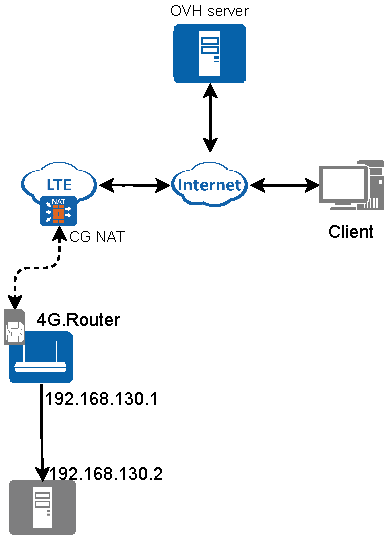
\includegraphics[width=0.44\linewidth]{immagini/diag2-host_real}
    }
    \begin{subfigure}{0.44\linewidth}
        \centering
        \usebox{\myimage}
        \caption{Diagramma di stato degli host domotici}
        \label{fig:diag2-host}
    \end{subfigure}
    \hfill
    \begin{subfigure}{0.53\linewidth}
        \centering
        \raisebox{\dimexpr.5\ht\myimage-.6\height\relax}{
            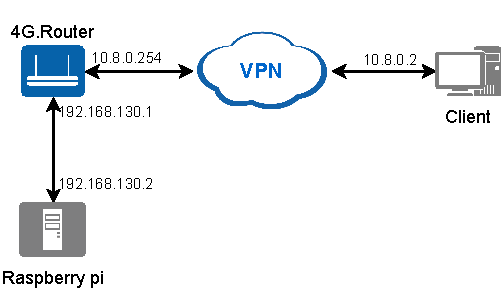
\includegraphics[width=1\linewidth]{immagini/diag2-host_virtual}
        }
        \caption{Diagramma di stato degli host domotici}
        \label{fig:diag2-host1}
    \end{subfigure}
\end{figure}

\section{Creazione della firewall zone per la VPN} 

Per rendere possibile la comunicazione tra la rete \it{lan} del \it{Router} e la VPN e' necessario configurare opportunamente il firewall.

Cio' viene fatto direttamente da luci, nella sezione firewall si avranno preconfigurate 2 zone, lan e wan, come si vede figura \ref{fig:luci-firewall-init}.

\begin{figure}[H]
    \centering
    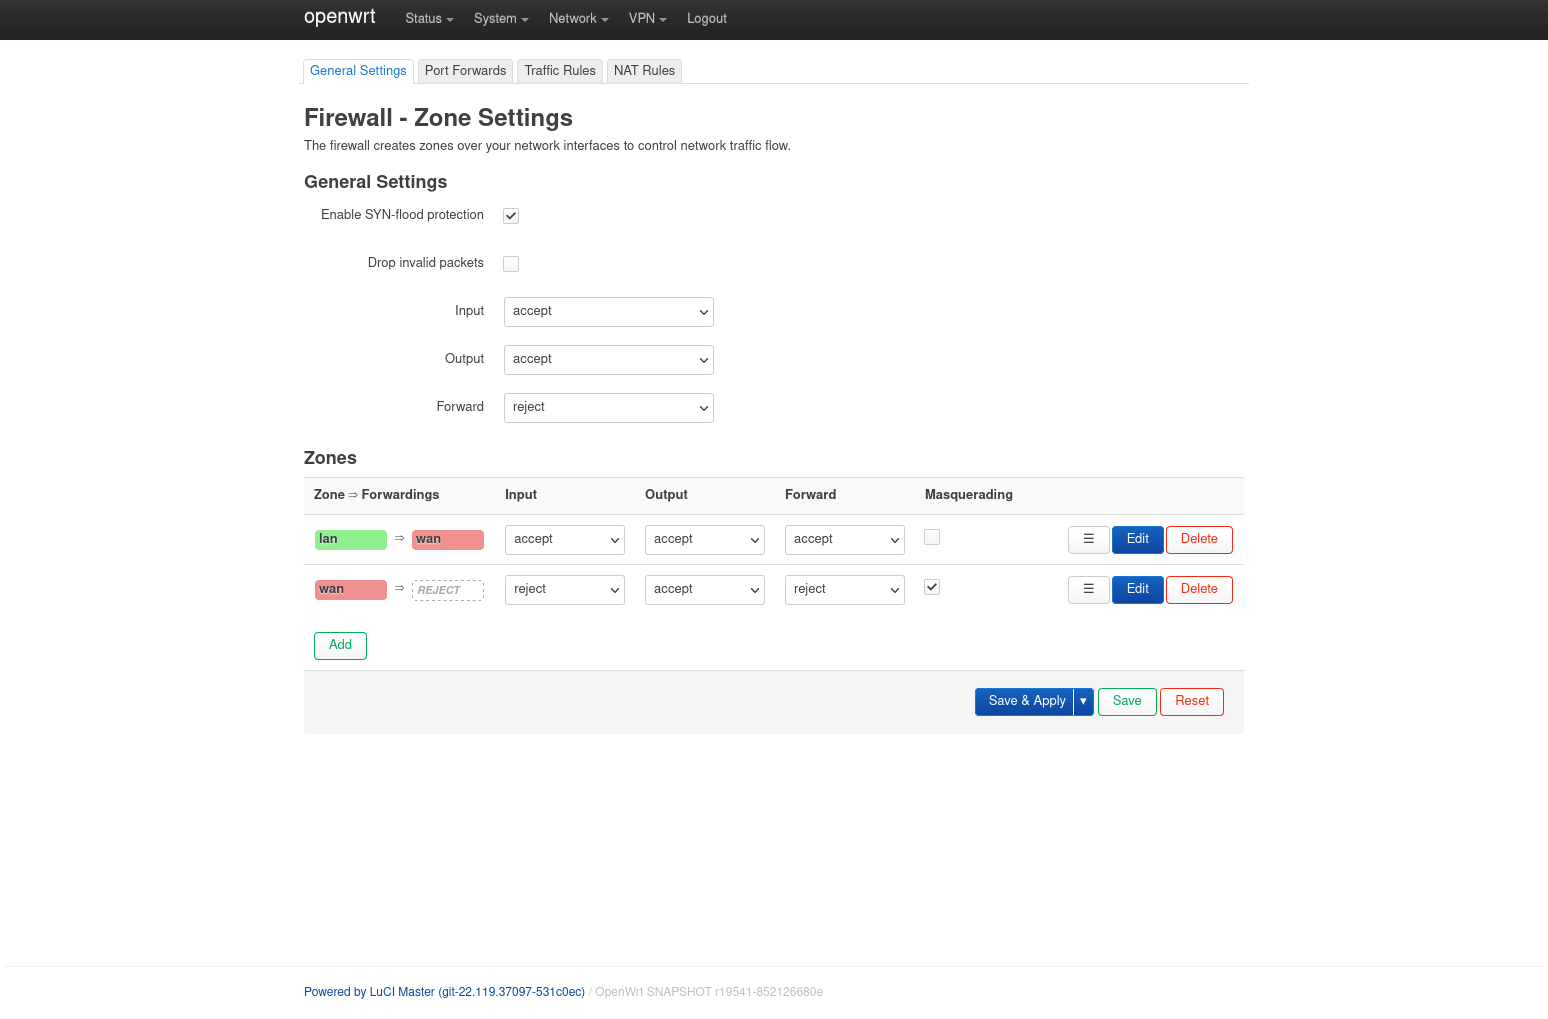
\includegraphics[width=0.9\linewidth]{immagini/LuCI_firewall_init}
    \caption{Configurazione iniziale del firewall}
    \label{fig:luci-firewall-init}
\end{figure}

Si deve quindi aggiungere una nuova zona, chiamata vpn, con le seguenti opzioni:
\begin{itemize}
    \item Policy di forward: accept
    \item Forward consentito verso la zona lan
    \item Forward consentito dalla zona lan
\end{itemize}

Possiamo vedere la pagina di configurazione:

\begin{figure}[H]
    \centering
    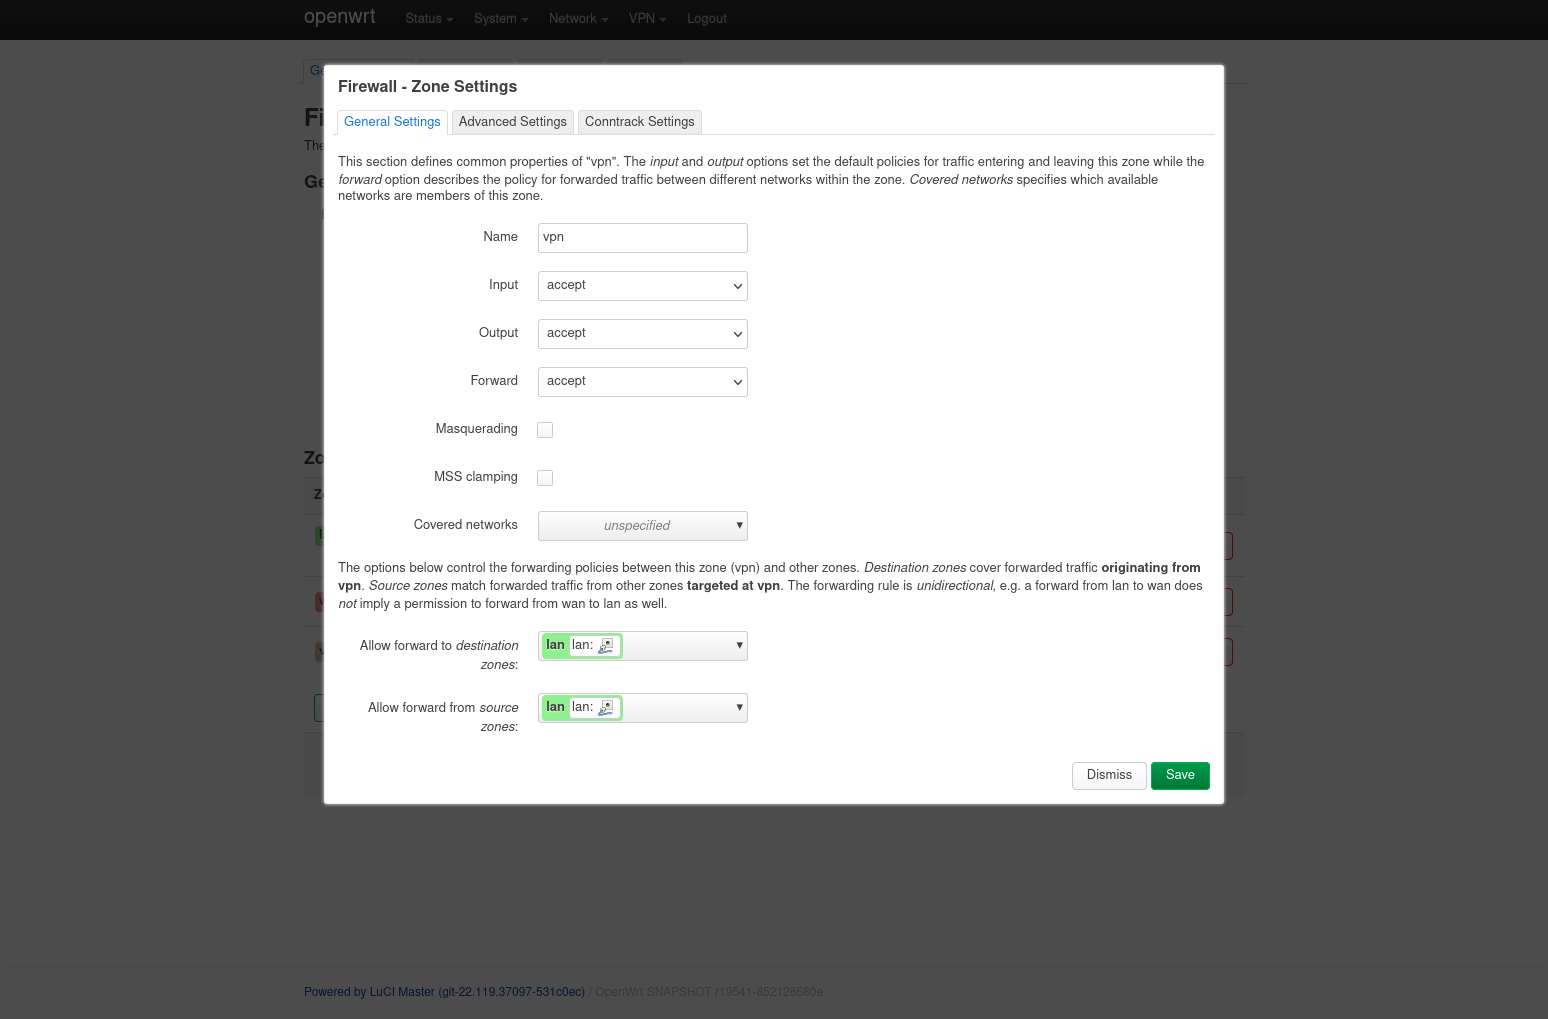
\includegraphics[width=0.9\linewidth]{immagini/LuCI_firewall_vpn}
    \caption{Configurazione del firewall}
    \label{fig:luci-firewall-vpn}
\end{figure}

Dopo aver salvato, la pagina del firewall sara':

\begin{figure}[H]
    \centering
    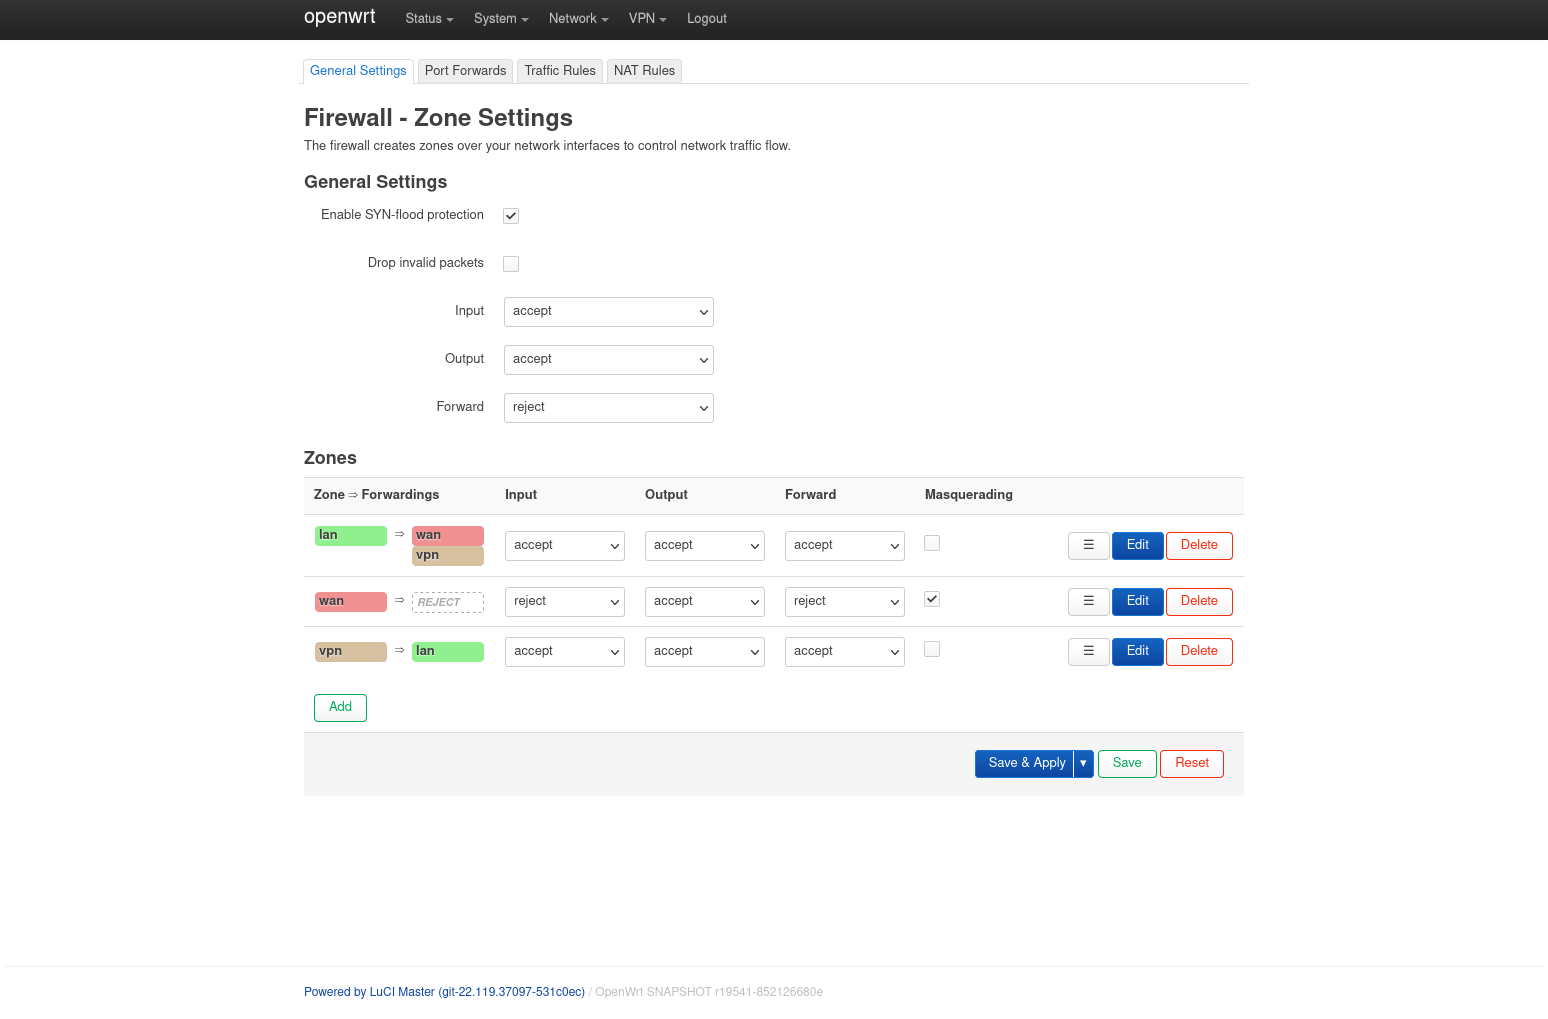
\includegraphics[width=0.9\linewidth]{immagini/LuCI_firewall_end}
    \caption{Configurazione finale del firewall}
    \label{fig:luci-firewall-end}
\end{figure}

\section{Aggiunta dell'interfaccia tun0 alla zona vpn}

Per rendere attiva la zona firewall appena creata gli si deve assegnare almeno un'interfaccia, in questo caso gli si deve assegnare l'interfaccia tun0.

Cio' va fatto da luci, nella sezione \it{interfaces}. Si deve quindi aggiungere una nuova interfaccia con le seguenti opzioni:
\begin{itemize}
    \item Name: tun0
    \item Proto: static
    \item Device: tun0
    \item ipv4 address: 10.8.0.254
    \item ipv4 netmask: 255.255.255.0
    \item Assign firewall zone: vpn
\end{itemize}

\begin{figure}[H]
    \centering
    \begin{subfigure}{0.9\linewidth}
        \centering
        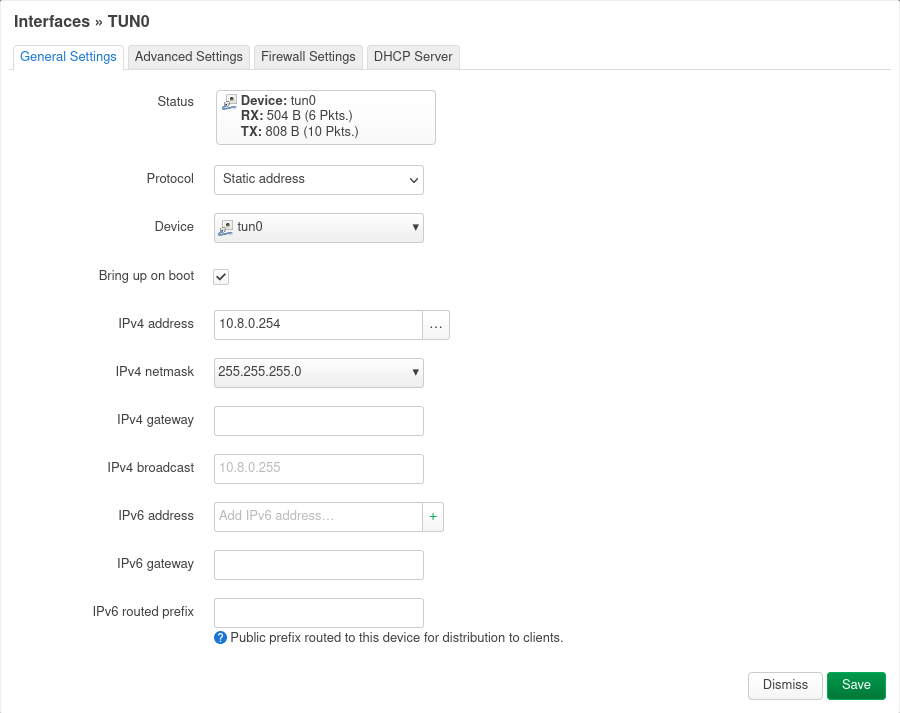
\includegraphics[width=0.7\linewidth]{immagini/LuCI_int_tun0_1}
        \caption{General settings}
        \label{fig:luci-firewall-interfaces}
    \end{subfigure}

    \begin{subfigure}{0.9\linewidth}
        \centering
        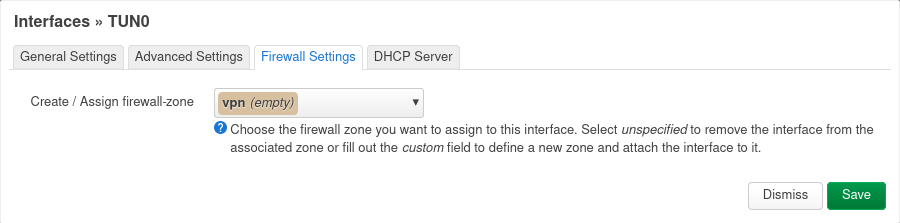
\includegraphics[width=0.7\linewidth]{immagini/LuCI_int_tun0_2}
        \caption{Firewall settings}
        \label{fig:luci-firewall-interfaces1}
    \end{subfigure}
\end{figure}


\section{Modifiche alla configurazione OpenVPN del server}

Per instaurare una comunicazione bidirezionale tra \it{host-domotico} e \it{clien} e' necessario che:

\begin{enumerate}
    \item il server vpn sia consapevole che il \it{router} vuole esporre una sua sottorete verso la vpn
    \item il client abbia l'opportuna rotta per raggiungere la sottorete dove si trova l'\it{host-domotico}
\end{enumerate}




Per il punto 2 e' necessario aggiungere la seguente riga alla configurazione OpenVPN nel \it{Server}:

\begin{bashcode}{Server}{}
$ vim /etc/openvpn/server/server.conf
168 push "route 192.168.130.0 255.255.255.0"
\end{bashcode}

In questo modo nel \it{client1} verra' aggiunta una nuova rotta nel momento in cui si connette alla vpn:

\begin{bashcode}{Client}{}
$ ip route
[...]
192.168.130.0/24 via 10.8.0.1 dev tun0
\end{bashcode}